	
	\subsection*{1.}
	
\begin{center}
	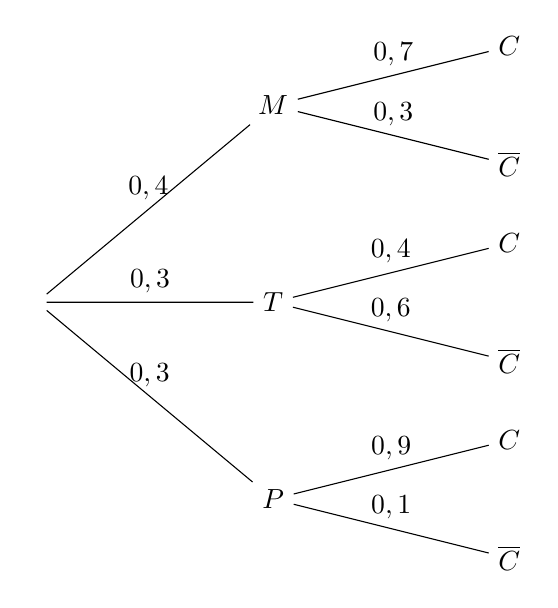
\begin{tikzpicture}
		[level 1/.style={level distance=3cm,
			sibling distance=2.5cm},
		level 2/.style={level distance=3cm,
			sibling distance=1.5cm}
		]
		\node {} [grow'=right]
		child {node {$M$}
			child {node {$C$}
				edge from parent node[above] {$0,7$}
			}
			child {node {$\overline C$}
				edge from parent node[above] {$0,3$}
			}
			edge from parent node[above] {$0,4$}
		}
		child {node {$T$}
			child {node {$C$}
				edge from parent node[above] {$0,4$}
			}
			child {node {$\overline C$}
				edge from parent node[above] {$0,6$}
			}
			edge from parent node[above] {$0,3$}
		}
		child {node {$P$}
			child {node {$C$}
				edge from parent node[above] {$0,9$}
			}
			child {node {$\overline C$}
				edge from parent node[above] {$0,1$}
			}
			edge from parent node[above] {$0,3$}
		}
		;
	\end{tikzpicture}
\end{center}
	
	\subsection*{2.}
	
	\[
	\begin{aligned}
		&P(T \cap C) = P(T) \times P_T(C) = 0,3 \times 0,4 = 0,12, \\
		&P(M \cap C) = P(M) \times P_M(C) = 0,4 \times 0,7 = 0,28, \\
		&P(P \cap C) = P(P) \times P_P(C) = 0,3 \times 0,9 = 0,27.
	\end{aligned}
	\]
	
	D’après la loi des probabilités totales :
	\[
	P(C) = P(T \cap C) + P(M \cap C) + P(P \cap C) = 0,12 + 0,28 + 0,27 = 0,67.
	\]
	
	\subsection*{3.}
	
	Il faut trouver \(P_C(T)\) :
	\[
	P_C(T) = \dfrac{P(C \cap T)}{P(C)} = \dfrac{P(T \cap C)}{P(C)} = \dfrac{0,12}{0,67} = \dfrac{12}{67}.
	\]
	
